\mode<presentation>
{
  \usetheme{CambridgeUS}
  \usecolortheme{whale}
  \usecolortheme{lily}

  \setbeamercovered{transparent}
  \usefonttheme[onlymath]{serif}
}

\title[\ModelingMechanicalSystemsShortName] % (optional, use only with long paper titles)
{\course: \ModelingMechanicalSystemsName\license}

\subtitle
{Lecture \ModelingMechanicalSystemsNumber} % (optional)



\begin{document}

\begin{frame}
  \titlepage
\end{frame}

\mode<article>{
\maketitle
\tableofcontents
}

%\mode<presentation>{
%\begin{frame}{Outline}
%  \tableofcontents
%  % You might wish to add the option [pausesections]
%\end{frame}}
\section{Pre-requisite Material}
This lecture assumes that the reader is familiar with the following material:
\begin{itemize}
\item Algebraic equations
\item Differential equations
\item Mechanics - Newton's law of motion, spring and damping forces
\end{itemize}


\section{Modeling}

\subsection{The Objective of Modeling}

Almost all feedback control systems have a common framework for implementation. As shown below, the ``plant'' contains two parts: the system to be controlled, and the actuator, which can take signals sent to it by the controller and convert them to actions. A sensor takes measurements of the plant, which are compared to a reference. The error between the reference command and actual output is supplied to a controller, which then decides on the signal that should be sent to the actuator, completing the loop.

\begin{frame}{Feedback Control System}
\begin{center}
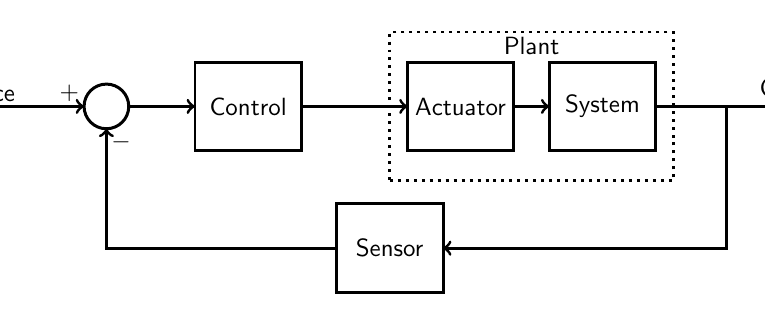
\begin{tikzpicture}[inner sep=0pt,outer sep=0pt,very thick,
sysblock/.style={draw,rectangle,inner sep=2pt,minimum width=1.5cm,minimum height=1.25cm,very thick}]
\useasboundingbox (-1,1) rectangle (8,-2.5); 
\begin{scope}[transform canvas={scale=.9}]
\draw (0,0) node[draw,circle] (sum) {$\rule{0pt}{18pt}$};
\draw (2,0) node[sysblock] (C) {\textsf{Control}};
\draw (5,0) node[sysblock] (A) {\textsf{Actuator}};
\draw (7,0) node[sysblock] (G) {\textsf{System}};
\draw (6,0) node[draw,rectangle,dotted,minimum width=4cm,minimum height=2.1cm] {};
\draw (6,.85) node {\textsf{Plant}};
\draw (4,-2) node[sysblock] (H) {\textsf{Sensor}};

\draw[->] (-2,0) node[above=2pt] {\textsf{Reference}} -- (sum.180) node[above left=2pt] {$+$};
\draw[->] (sum.0) -- (C);
\draw[->] (C) -- (A);
\draw[->] (A) -- (G);
\draw[->] (G.0) -- ++(2,0) node[above=2pt] {\textsf{Output}};
\draw[->] (G.0) -- ++(1,0) |- (H);
\draw[->] (H) -| (sum.-90) node[below right=2pt] {$-$};
\end{scope}
\end{tikzpicture}

\end{center}
\end{frame}

As an example, consider the feedback system created by a room thermostat

\begin{frame}{Thermostat Feedback Control System\footnote{\tiny Images: Amanitamano (Own work) [CC-BY-SA-3.0],  Paul Robinson (New Image) [CC-BY-SA-3.0], via Wikimedia Commons  }}
\begin{center}
\mode<article>{\input{figures/controlsystemsetup2.tex}}
\mode<presentation>{\resizebox{3in}{!}{\input{figures/controlsystemsetup2.tex}}}
\end{center}
\end{frame}

The plant in this case consists of the room, along with the actuator that is the cooling or heating device. The thermostat receives a desired setpoint from the user, along with the actual temperature as measured using a temperature sensor, and then determines how to actuate the cooling or heating device based on a control law.

\begin{framed}
Different plants have different behavior. In order to design a control system that decides what the input should be, we need to be able to {\em predict} how that plant will respond to different inputs. This is the purpose of a model.
\end{framed}

For the thermostat, the required model is fairly simple (i.e., if I send out a signal to turn on the air conditioner, the temperature will decrease), but for many dynamical systems, relationship between the input of the plant and the output can be much more complicated.

\subsection{Lumped Modeling using Idealized Components}

In order to model a system, we have to answer a few questions. Consider a suspension system on an automobile, as shown below. The suspension system consists of several different components that are connected together. These components include the tire (and axle), the spring, the shock absorber (damper), and the car chassis. What would a model of this system be?
%\begin{frame}{Modeling}
\begin{itemize}
\item What signals are we interested in? Any physical system has many attributes - In this case, we want to know the translational motion of each element of the suspension system. Other attributes, for example, the temperature of each component, are not of interest.
\item What is the desired level of accuracy? Do we want to know just the relative motion in the plane, or are we also interested in the flexible motion of the components (vibrations)?
\item What is the time scale? 
\end{itemize}
%\end{frame}
\begin{frame}{Components of an automobile suspension\footnote{{\tiny Images: By Bukk (Own work) [Public domain], via Wikimedia Commons}}}
\begin{center}
\includegraphics[width=2.3in]{figures/Federbein_Seicentosuspension_small}\input{figures/autosuspension.tex}
\end{center}

\end{frame}\vspace{.1in}

The simplest type of modeling is {\em lumped} modeling, where we only keep track of variables such as position or velocity at the connections between components, which will result in a series of ordinary differential equations. This is the kind of modeling that we will focus on in this class. In order to develop our equations, we will use interconnections of {\em idealized elements} that express one specific type of behavior. 

The types of systems and idealized elements that we will be using are given in the following table.

\begin{frame}{Modeling Domains and Idealized Elements}
\begin{center}
\mode<article>{\begin{tabular}{p{2.5in}p{2.5in}}}
\mode<presentation>{\begin{tabular}{p{2.2in}p{2.2in}}}
System Class & Idealized Elements  \\\hline\hline
Mechanical Systems, Translational Motion & Mass, Spring, Damper \\\hline
Mechanical Systems, Rotational Motion & Inertia, Spring, Damper \\\hline
Electrical Systems & Resistor, Capacitor, Inductor \\\hline
Fluid Systems & Tank, Valve \\\hline
Thermal Systems & Thermal Capacitance, Thermal Resistance \\ 
\end{tabular}
\end{center}
\end{frame}

%What are mechanical systems? Control of \underline{motion} \\
% Examples:
% \begin{itemize} 
%\item Automobile cruise control and stability control 
%\item Satellite orientation 
%\item Aircraft 
%\item  Active damping for buildings and large trusses 
%\item  Cranes 
%\item  Rockets
%\end{itemize}   



\section[Idealized Components]{Idealized components for translational motion of mechanical systems}
We will use the following elements to describe translational mechanical systems. The variables that we are modeling are 
\mode<article>{\begin{frame}}
\mode<presentation>{\begin{frame}{Modeling variables for translational motion}}
\begin{itemize}
\item \visible<2->{force, which has units of Newtons [N],}
\item \visible<2->{position, which has units of meters [m].}
\end{itemize}
\end{frame}
Unless otherwise specified, we will always assume that the force and position variables have these units. We will see that the differential equations that describe a mechanical system arrive from the relationships {\em between} these variables. 
\begin{frame}
\begin{definition}
The laws that describe the relationship between position (or velocity, or acceleration) and force on an ideal element are called the {\em component model}, or constitutive relationship. 
\end{definition}
\end{frame}
The component models for the mechanical ideal elements are given in the next sections

\subsection{Mass}
As familiar from physics, all objects have mass, which relates the applied force to the acceleration of that object through Newton's Law. In this diagram, we have illustrated two forces that are acting on the mass, but there could be more or fewer. 
\mode<presentation>{\begin{frame}{Idealized Mass}}
\mode<article>{\begin{frame}}
\begin{center}
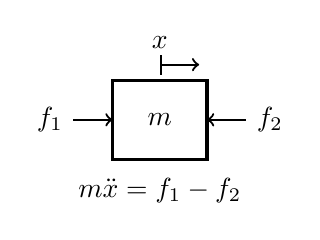
\begin{tikzpicture}
    \draw[very thick] (0,0) rectangle (1.2,1);
    \draw (.6,.5) node {$m$};
    \draw[<-,thick] (1.2,.5) -- ++(.5,0) node[right] {$f_{2}$};
    \draw[<-,thick] (0,.5) -- ++(-.5,0) node[left] {$f_{1}$};
    \draw[|->,thick] (.6,1.2) node[above=2pt] {$x$} -- ++(.5,0);  
        \draw<2-> (.6,-.4) node {$m\ddot{x}=f_{1}-f_{2}$};

\end{tikzpicture}

\end{center}
\mode<article>{Note that we are using the dot notation for derivative with respect to time, for example}
\visible<2->{\begin{equation*}
\dot{x}\equiv \frac{dx}{dt},\quad \ddot{x} \equiv \frac{d^{2}x}{dt^{2}},\quad \dots.
\end{equation*}}%
\end{frame}

Newton's law sums the applied forces, with the sign depending on whether the force is in the same direction or opposition direction as positive position. 
In this context, the mass of an object is simply a scaling factor between force and acceleration. Given the units that we have defined for position and force, the units of mass are [N s$^{2}$ m$^{-1}$]. However, in SI units, this is defined to be the kilogram, or [kg]. 

\noindent\textbf{A Note on Notation:} We have used the notation 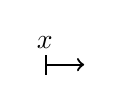
\begin{tikzpicture}  \draw(0,0)[|->,thick] node[above=2pt]{$x$} -- ++(.5,0); \end{tikzpicture} to indicate that we are going to measure the position of the mass with the variable $x$ (in meters), with $x$ positive indicating that the mass has moved to the right. However, this is still a bit ambiguous - moved to the right with respect to what? We need to specify a non-accelerating {\em fixed point} that all positions are measured with respect to - this is called a ground. So really, our picture should look like the following:
\mode<presentation>{\begin{frame}{Positions are measured with respect to fixed point}}
\mode<article>{\begin{frame}}
\begin{center}
\begin{tikzpicture}
%  \draw(-1,2.5) node (text) {\textsf{fixed point}};
%   \draw[->] (text.180) -- ++(-.7,0);
   \draw[inner sep=0pt,outer sep=0pt,very thick] (-3,1) node (gnd1) {\input{\mainfolder/DrawingElements/MechanicalElements/ground.tex}};
   \draw[->|,dotted] (-3,1.75) -- node[pos=.5,above] {$x_{f}$} ++(3.6,0); 
    \draw[very thick] (0,0) rectangle (1.2,1);
    \draw (.6,.5) node {$m$};
    \draw[->,thick] (1.2,.5) -- ++(.5,0) node[right] {$f$};
    \draw[|->,thick] (.6,1.2) node[above=2pt] {$x$} -- ++(.5,0);  
\end{tikzpicture}

\end{center}
\[
\frac{d^2(x_{f}+x)}{dt^2} = \frac{d^2x}{dt^2} 
\]
\end{frame} 
Note that the point where $x=0$ is a fixed point with respect to ground. So it would be most correct to say ``The position of the mass is $x_{f}$ plus $x$''. In our analysis, because we are working with elements that have linear relationships, we can always subtract off this fixed distance and measure positions with $x$ alone. So in what follows, we will simply say ``The position of the mass is $x$.''

\subsection{Damper}
When the engine applies a force to your car, it will accelerate, but only up to a point. Eventually drag forces, or other friction forces, will oppose the force applied by the car. This is modeled by a damper. The relative velocity of the ends of the damper is proportional to the applied force.
\mode<presentation>{\begin{frame}{Idealized Damper}}
\mode<article>{\begin{frame}}
\begin{center}
\begin{tikzpicture}
\draw[very thick] (-.2,0) -- (0,0);
\draw (.75,0) node {\begin{tikzpicture}
\draw[very thick] (-.2,0) -- (0,0);
\draw (.75,0) node {\begin{tikzpicture}
\draw[very thick] (-.2,0) -- (0,0);
\draw (.75,0) node {\input{\mainfolder/DrawingElements/MechanicalElements/damper.tex}};
\draw (.75,0) node[above=9pt] {$b$};
\draw[very thick] (1.5,0) -- ++(.2,0);
    \draw[<-,thick] (1.5,0) ++(.2,0) -- ++(.5,0) node[right] {$f$};
    \draw[<-,thick] (-.2,0) -- ++(-.5,0) node[left] {$f$};
    \draw[|->,thick] (-.2,.4) node[above=2pt] {$x_{1}$} -- ++(.5,0);  
    \draw[|->,thick] (1.7,.4) node[above=2pt] {$x_{2}$} -- ++(.5,0);  
    \draw (.6,-.6) node {$x=x_{1}-x_{2}$};
  %  \draw (.6,-1.2) node {$f=b\dot{x}$};
\end{tikzpicture}};
\draw (.75,0) node[above=9pt] {$b$};
\draw[very thick] (1.5,0) -- ++(.2,0);
    \draw[<-,thick] (1.5,0) ++(.2,0) -- ++(.5,0) node[right] {$f$};
    \draw[<-,thick] (-.2,0) -- ++(-.5,0) node[left] {$f$};
    \draw[|->,thick] (-.2,.4) node[above=2pt] {$x_{1}$} -- ++(.5,0);  
    \draw[|->,thick] (1.7,.4) node[above=2pt] {$x_{2}$} -- ++(.5,0);  
    \draw (.6,-.6) node {$x=x_{1}-x_{2}$};
  %  \draw (.6,-1.2) node {$f=b\dot{x}$};
\end{tikzpicture}};
\draw (.75,0) node[above=9pt] {$b$};
\draw[very thick] (1.5,0) -- ++(.2,0);
    \draw[<-,thick] (1.5,0) ++(.2,0) -- ++(.5,0) node[right] {$f$};
    \draw[<-,thick] (-.2,0) -- ++(-.5,0) node[left] {$f$};
    \draw[|->,thick] (-.2,.4) node[above=2pt] {$x_{1}$} -- ++(.5,0);  
    \draw[|->,thick] (1.7,.4) node[above=2pt] {$x_{2}$} -- ++(.5,0);  
    \draw (.6,-.6) node {$x=x_{1}-x_{2}$};
  %  \draw (.6,-1.2) node {$f=b\dot{x}$};
\end{tikzpicture}
\end{center}
\end{frame}
Note that the applied force is always {\em equal and opposite} on both ends of the damper. Since this is an ``ideal'' damper, it contains no mass, and thus it cannot sustain a net force, otherwise it would sustain infinite acceleration. By unit analysis, the units of the damping constant $b$ are [N s m$^{-1}$].

\subsection{Spring}
The final behavior we will model is elastic compressibility. The ideal element is the linear spring. Relative compression between the ends of the spring is proportional to the applied force.
\mode<presentation>{\begin{frame}{Idealized Spring}}
\mode<article>{\begin{frame}}\begin{center}
\begin{tikzpicture}
\draw (.75,0) node[inner sep=0,outer sep=0] (K1) {\begin{tikzpicture}
\draw (.75,0) node[inner sep=0,outer sep=0] (K1) {\begin{tikzpicture}
\draw (.75,0) node[inner sep=0,outer sep=0] (K1) {\input{\mainfolder/DrawingElements/MechanicalElements/spring.tex}};
\draw (K1)  node[above=6pt] {$k$};
\draw[very thick] (K1.180) -- ++(-.2,0);
\draw[very thick] (K1.0) -- ++(0.2,0);
\draw[<-,thick] (K1.0) ++(.2,0) -- ++(.5,0) node[right] {$f$};
\draw[<-,thick] (K1.180) ++(-.2,0) -- ++(-.5,0) node[left] {$f$};
\draw[|->,thick] (K1.180) ++(-.2,.4) node[above=2pt] {$x_{1}$} -- ++(.5,0);  
\draw[|->,thick] (K1.0) ++(.2,.4) node[above=2pt] {$x_{2}$} -- ++(.5,0);  
\draw<2-> (K1) ++(0,-.6) node {$f=k(x_{1}-x_{2})$};
\end{tikzpicture}
};
\draw (K1)  node[above=6pt] {$k$};
\draw[very thick] (K1.180) -- ++(-.2,0);
\draw[very thick] (K1.0) -- ++(0.2,0);
\draw[<-,thick] (K1.0) ++(.2,0) -- ++(.5,0) node[right] {$f$};
\draw[<-,thick] (K1.180) ++(-.2,0) -- ++(-.5,0) node[left] {$f$};
\draw[|->,thick] (K1.180) ++(-.2,.4) node[above=2pt] {$x_{1}$} -- ++(.5,0);  
\draw[|->,thick] (K1.0) ++(.2,.4) node[above=2pt] {$x_{2}$} -- ++(.5,0);  
\draw<2-> (K1) ++(0,-.6) node {$f=k(x_{1}-x_{2})$};
\end{tikzpicture}
};
\draw (K1)  node[above=6pt] {$k$};
\draw[very thick] (K1.180) -- ++(-.2,0);
\draw[very thick] (K1.0) -- ++(0.2,0);
\draw[<-,thick] (K1.0) ++(.2,0) -- ++(.5,0) node[right] {$f$};
\draw[<-,thick] (K1.180) ++(-.2,0) -- ++(-.5,0) node[left] {$f$};
\draw[|->,thick] (K1.180) ++(-.2,.4) node[above=2pt] {$x_{1}$} -- ++(.5,0);  
\draw[|->,thick] (K1.0) ++(.2,.4) node[above=2pt] {$x_{2}$} -- ++(.5,0);  
\draw<2-> (K1) ++(0,-.6) node {$f=k(x_{1}-x_{2})$};
\end{tikzpicture}

\end{center}
\end{frame}
Like the damper, the applied force is always {\em equal and opposite} on both ends of the spring. By unit analysis, the units of the spring constant $k$ are [N m$^{-1}$].


\subsection{Connection Rules}

%We can build a more complex system by attaching ideal elements to each other. There are two connection rules to follow. For example, suppose we connect a spring to a damper.
%\begin{frame}{Connecting a Spring and Damper}
%\begin{center}
%\begin{tikzpicture}[inner sep=0pt,outer sep=0pt,very thick]
\draw (1,0) node (gnd) {\input{\mainfolder/DrawingElements/MechanicalElements/ground.tex}};
\draw (3.5,0.5) node (K1) {\begin{tikzpicture}
\draw (.75,0) node[inner sep=0,outer sep=0] (K1) {\begin{tikzpicture}
\draw (.75,0) node[inner sep=0,outer sep=0] (K1) {\input{\mainfolder/DrawingElements/MechanicalElements/spring.tex}};
\draw (K1)  node[above=6pt] {$k$};
\draw[very thick] (K1.180) -- ++(-.2,0);
\draw[very thick] (K1.0) -- ++(0.2,0);
\draw[<-,thick] (K1.0) ++(.2,0) -- ++(.5,0) node[right] {$f$};
\draw[<-,thick] (K1.180) ++(-.2,0) -- ++(-.5,0) node[left] {$f$};
\draw[|->,thick] (K1.180) ++(-.2,.4) node[above=2pt] {$x_{1}$} -- ++(.5,0);  
\draw[|->,thick] (K1.0) ++(.2,.4) node[above=2pt] {$x_{2}$} -- ++(.5,0);  
\draw<2-> (K1) ++(0,-.6) node {$f=k(x_{1}-x_{2})$};
\end{tikzpicture}
};
\draw (K1)  node[above=6pt] {$k$};
\draw[very thick] (K1.180) -- ++(-.2,0);
\draw[very thick] (K1.0) -- ++(0.2,0);
\draw[<-,thick] (K1.0) ++(.2,0) -- ++(.5,0) node[right] {$f$};
\draw[<-,thick] (K1.180) ++(-.2,0) -- ++(-.5,0) node[left] {$f$};
\draw[|->,thick] (K1.180) ++(-.2,.4) node[above=2pt] {$x_{1}$} -- ++(.5,0);  
\draw[|->,thick] (K1.0) ++(.2,.4) node[above=2pt] {$x_{2}$} -- ++(.5,0);  
\draw<2-> (K1) ++(0,-.6) node {$f=k(x_{1}-x_{2})$};
\end{tikzpicture}
};
\draw (K1) node[above=14pt] {$k$};
\draw (3.5,-0.5) node (B1) {\begin{tikzpicture}
\draw[very thick] (-.2,0) -- (0,0);
\draw (.75,0) node {\begin{tikzpicture}
\draw[very thick] (-.2,0) -- (0,0);
\draw (.75,0) node {\input{\mainfolder/DrawingElements/MechanicalElements/damper.tex}};
\draw (.75,0) node[above=9pt] {$b$};
\draw[very thick] (1.5,0) -- ++(.2,0);
    \draw[<-,thick] (1.5,0) ++(.2,0) -- ++(.5,0) node[right] {$f$};
    \draw[<-,thick] (-.2,0) -- ++(-.5,0) node[left] {$f$};
    \draw[|->,thick] (-.2,.4) node[above=2pt] {$x_{1}$} -- ++(.5,0);  
    \draw[|->,thick] (1.7,.4) node[above=2pt] {$x_{2}$} -- ++(.5,0);  
    \draw (.6,-.6) node {$x=x_{1}-x_{2}$};
  %  \draw (.6,-1.2) node {$f=b\dot{x}$};
\end{tikzpicture}};
\draw (.75,0) node[above=9pt] {$b$};
\draw[very thick] (1.5,0) -- ++(.2,0);
    \draw[<-,thick] (1.5,0) ++(.2,0) -- ++(.5,0) node[right] {$f$};
    \draw[<-,thick] (-.2,0) -- ++(-.5,0) node[left] {$f$};
    \draw[|->,thick] (-.2,.4) node[above=2pt] {$x_{1}$} -- ++(.5,0);  
    \draw[|->,thick] (1.7,.4) node[above=2pt] {$x_{2}$} -- ++(.5,0);  
    \draw (.6,-.6) node {$x=x_{1}-x_{2}$};
  %  \draw (.6,-1.2) node {$f=b\dot{x}$};
\end{tikzpicture}};
\draw (B1) node[below=14pt] {$b$};


\draw (K1.180) -- (K1.180 -| gnd.0);
\draw (B1.180) -- (B1.180 -| gnd.0);
\draw (K1.0) -- ++(0.5,0) |- ++(1,-.5) node[circle,fill,inner sep=0] (F) {\rule{0pt}{4pt}};
\draw (B1.0) -- ++(0.5,0) |- ++(0,.5);
\draw[|->,thick] (F) ++(0,.5) node[above=6pt] {$x$} -- ++(.5,0);
\draw[->,thick] (F) -- ++(.75,0) node[right=2pt] {$f_{in}$}; 

\end{tikzpicture}
%\end{center}
%\end{frame}
%
%\begin{itemize}
%\item When two elements are connected, the two components share the same {\em position}. Thus, in the above example 
%\[
%x_{2}=x_{3}
%\]
%is a connection constraint
%\item When two elements are connected, the forces at the connection {\em sum to zero} (keeping track of direction). Thus, in the above example \[
%f_{k}=f_{b}
%\]
%since they point is opposite directions.
%\end{itemize}
%
%\subsection{Boundary Conditions}
%
%Often, we will want to prescribe either the position or force of a particular terminal. For example, consider the following two diagrams
%
%\begin{frame}{Applying Boundary Conditions}
%\begin{center}
%\begin{tikzpicture}

\draw[inner sep=0pt,outer sep=0pt,very thick] (-4,0) node (gnd1) {\input{\mainfolder/DrawingElements/MechanicalElements/ground.tex}};
\draw[inner sep=0pt,outer sep=0pt,very thick] (-2,0) node (K1) {\begin{tikzpicture}
\draw (.75,0) node[inner sep=0,outer sep=0] (K1) {\begin{tikzpicture}
\draw (.75,0) node[inner sep=0,outer sep=0] (K1) {\input{\mainfolder/DrawingElements/MechanicalElements/spring.tex}};
\draw (K1)  node[above=6pt] {$k$};
\draw[very thick] (K1.180) -- ++(-.2,0);
\draw[very thick] (K1.0) -- ++(0.2,0);
\draw[<-,thick] (K1.0) ++(.2,0) -- ++(.5,0) node[right] {$f$};
\draw[<-,thick] (K1.180) ++(-.2,0) -- ++(-.5,0) node[left] {$f$};
\draw[|->,thick] (K1.180) ++(-.2,.4) node[above=2pt] {$x_{1}$} -- ++(.5,0);  
\draw[|->,thick] (K1.0) ++(.2,.4) node[above=2pt] {$x_{2}$} -- ++(.5,0);  
\draw<2-> (K1) ++(0,-.6) node {$f=k(x_{1}-x_{2})$};
\end{tikzpicture}
};
\draw (K1)  node[above=6pt] {$k$};
\draw[very thick] (K1.180) -- ++(-.2,0);
\draw[very thick] (K1.0) -- ++(0.2,0);
\draw[<-,thick] (K1.0) ++(.2,0) -- ++(.5,0) node[right] {$f$};
\draw[<-,thick] (K1.180) ++(-.2,0) -- ++(-.5,0) node[left] {$f$};
\draw[|->,thick] (K1.180) ++(-.2,.4) node[above=2pt] {$x_{1}$} -- ++(.5,0);  
\draw[|->,thick] (K1.0) ++(.2,.4) node[above=2pt] {$x_{2}$} -- ++(.5,0);  
\draw<2-> (K1) ++(0,-.6) node {$f=k(x_{1}-x_{2})$};
\end{tikzpicture}
};

\draw[very thick] (gnd1.0) -- (K1.180);
\draw[very thick] (K1.0) -- ++(1,0) node (input) {};
\draw[|->] (input) ++(0,.25) node[above] {$x_{in}$} -- ++(-.5,0);

\draw[inner sep=0pt,outer sep=0pt,very thick] (2,0) node (gnd2) {\input{\mainfolder/DrawingElements/MechanicalElements/ground.tex}};
\draw[inner sep=0pt,outer sep=0pt,very thick] (4,0) node (K2) {\begin{tikzpicture}
\draw (.75,0) node[inner sep=0,outer sep=0] (K1) {\begin{tikzpicture}
\draw (.75,0) node[inner sep=0,outer sep=0] (K1) {\input{\mainfolder/DrawingElements/MechanicalElements/spring.tex}};
\draw (K1)  node[above=6pt] {$k$};
\draw[very thick] (K1.180) -- ++(-.2,0);
\draw[very thick] (K1.0) -- ++(0.2,0);
\draw[<-,thick] (K1.0) ++(.2,0) -- ++(.5,0) node[right] {$f$};
\draw[<-,thick] (K1.180) ++(-.2,0) -- ++(-.5,0) node[left] {$f$};
\draw[|->,thick] (K1.180) ++(-.2,.4) node[above=2pt] {$x_{1}$} -- ++(.5,0);  
\draw[|->,thick] (K1.0) ++(.2,.4) node[above=2pt] {$x_{2}$} -- ++(.5,0);  
\draw<2-> (K1) ++(0,-.6) node {$f=k(x_{1}-x_{2})$};
\end{tikzpicture}
};
\draw (K1)  node[above=6pt] {$k$};
\draw[very thick] (K1.180) -- ++(-.2,0);
\draw[very thick] (K1.0) -- ++(0.2,0);
\draw[<-,thick] (K1.0) ++(.2,0) -- ++(.5,0) node[right] {$f$};
\draw[<-,thick] (K1.180) ++(-.2,0) -- ++(-.5,0) node[left] {$f$};
\draw[|->,thick] (K1.180) ++(-.2,.4) node[above=2pt] {$x_{1}$} -- ++(.5,0);  
\draw[|->,thick] (K1.0) ++(.2,.4) node[above=2pt] {$x_{2}$} -- ++(.5,0);  
\draw<2-> (K1) ++(0,-.6) node {$f=k(x_{1}-x_{2})$};
\end{tikzpicture}
};

\draw[very thick] (gnd2.0) -- (K2.180);
\draw[very thick] (K2.0) -- ++(1,0) node[inner sep=0,outer sep=0] (input2) {};
\draw[<-] (input2) -- ++(.5,0) node[right] {$f_{in}$};


\draw(0,-3) node {\begin{tikzpicture}
\draw[very thick] (-.2,0) -- (0,0);
\draw (.75,0) node (K1) {\begin{tikzpicture}
\draw (.75,0) node[inner sep=0,outer sep=0] (K1) {\begin{tikzpicture}
\draw (.75,0) node[inner sep=0,outer sep=0] (K1) {\input{\mainfolder/DrawingElements/MechanicalElements/spring.tex}};
\draw (K1)  node[above=6pt] {$k$};
\draw[very thick] (K1.180) -- ++(-.2,0);
\draw[very thick] (K1.0) -- ++(0.2,0);
\draw[<-,thick] (K1.0) ++(.2,0) -- ++(.5,0) node[right] {$f$};
\draw[<-,thick] (K1.180) ++(-.2,0) -- ++(-.5,0) node[left] {$f$};
\draw[|->,thick] (K1.180) ++(-.2,.4) node[above=2pt] {$x_{1}$} -- ++(.5,0);  
\draw[|->,thick] (K1.0) ++(.2,.4) node[above=2pt] {$x_{2}$} -- ++(.5,0);  
\draw<2-> (K1) ++(0,-.6) node {$f=k(x_{1}-x_{2})$};
\end{tikzpicture}
};
\draw (K1)  node[above=6pt] {$k$};
\draw[very thick] (K1.180) -- ++(-.2,0);
\draw[very thick] (K1.0) -- ++(0.2,0);
\draw[<-,thick] (K1.0) ++(.2,0) -- ++(.5,0) node[right] {$f$};
\draw[<-,thick] (K1.180) ++(-.2,0) -- ++(-.5,0) node[left] {$f$};
\draw[|->,thick] (K1.180) ++(-.2,.4) node[above=2pt] {$x_{1}$} -- ++(.5,0);  
\draw[|->,thick] (K1.0) ++(.2,.4) node[above=2pt] {$x_{2}$} -- ++(.5,0);  
\draw<2-> (K1) ++(0,-.6) node {$f=k(x_{1}-x_{2})$};
\end{tikzpicture}
};

\draw (.75,0)  node[above=6pt] {$k$};
\draw[very thick] (1.5,0) -- ++(0.2,0);
    \draw[<-,thick] (1.5,0) ++(0.2,0) -- ++(.5,0) node[right] {$f_{k}$};
    \draw[<-,thick] (-.2,0) -- ++(-.5,0) node[left] {$f_{k}$};
    \draw[|->,thick] (-.2,.4) node[above=2pt] {$x_{1}$} -- ++(.5,0);  
    \draw[|->,thick] (1.7,.4) node[above=2pt] {$x_{2}$} -- ++(.5,0);  
 \end{tikzpicture}};


\end{tikzpicture}

%\end{center}
%\end{frame}
%On the left side of each diagram we have placed the ground, discussed earlier. When a ground is connected to an element, this fixes the position of that terminal at zero. Thus, for both the left and right diagrams we have
%\[
%x_{1} =0.
%\]
%In the left hand diagram, we have indicated that the position of one side of the spring will be specified by the signal $x_{in}$. Thus,
%\[
%x_{2} = -x_{in},
%\]
%since $x_{2}$ and $x_{in}$ are pointing is opposite directions. 
%Similarly, in the right hand diagram, we have indicated that the force applied to one side of the spring will be specified by the signal $f_{in}$. Thus
%\[
%f_{k} = f_{in}.
%\]
%
%\subsection{Writing the equations of motion}
%
%Using the component laws and connection laws, we can write the equations of motion for a lumped translational system. This is as simple as writing down all of the relevant laws, and then eliminating variables.

Usually we are interested in systems that are an interconnection of many ideal elements. We can derive the equations of motion for such a system if we keep track of the connection rules.

Consider the following system with applied force $u$. We want to find a differential equation that will allow us to predict the position $y$, between the damper and the spring.
\begin{frame}{Connection Law Example: Spring-Damper System with Input}
\begin{center}
\input{figures/springanddamperandground1.tex}
\end{center}
\end{frame}

We can start by drawing what is called a free-body-diagram. We simply draw each element separately, and assign labels to the relevant positions and forces acting on these elements.  
\begin{frame}
\begin{center}
\input{figures/springanddamperandground2.tex}
\end{center}
\end{frame}


For the spring/damper system given above we have
\begin{align*}
\mbox{Component Laws}&
\left\{ \begin{matrix} f_{k} = k(x_{1}-x_{2})\\
f_{b}  = b(\dot{x}_{3}-\dot{x}_{4})
\end{matrix}\right.
\end{align*}

At this point, the signals $u$\footnote{If you downloaded an earlier version of this lecture, you may notice we've replaced $r$ with $u$ for reasons that will become clear in future articles.} and $y$ do not yet appear, and we have many more unknowns than equations. We need to apply what we will call connection rules. This allows us to eliminate variables at connections, and to add boundary conditions. 

When two elements are connected, the position variables become {\em equal}, while the forces must be {\em equal and opposite}, according to Newton's third law. For the system above, we have
\begin{align*}
\mbox{Connection Laws}&\left\{\begin{matrix} f_{k}=f_{b}\\
x_{2}=x_{3} 
\end{matrix}\right.
\end{align*}
When we specify a specific variable or trajectory for a force or position, this is called a boundary condition. Note that a ground specifies that the position is fixed at zero.
\begin{align*}
\mbox{Boundary Conditions}&\left\{\begin{matrix}x_{1}=0\\
f_{b}=u \\
x_{2}=y
\end{matrix}\right.\end{align*}
These three sets of equations then constitute the equations of motion for this system. Let's count variables (signals) and equations. The variables are $x_{1},x_{2},x_{3},x_{4},f_{b},f_{k},u,y$, or 8 variables. We have 7 equations. We can thus eliminate all the variables except two. (When we have done things correctly, this elimination ability will always be the case.) To achieve our modeling objective, we want to get an equation that involves only the input signal $u$ and the output signal $y$. 

To proceed, we should attempt to eliminate all variables except $u$ and $y$. We can start by using the boundary conditions to replace $x_{1}$, $f_{b}$ and $x_{2}$ in the component laws and connection laws. This gives us
\begin{align*}
f_{k} &= -k(y),\\
u & = b(\dot{x}_{3}-\dot{x}_{4}),\\
f_{k}&=u,\\
y&=x_{3}. \
\end{align*}
Then, using the bottom two equations to replace $f_{k}$ and $x_{3}$ in the top two equations,
\begin{align*}
u &= -k(y),\\
u & = b(\dot{y}-\dot{x}_{4}).\
\end{align*}
Often, we will have to keep going until we get one equation. However, in this case, (because of the types of elements that are interconnected) we see that the first equation already gives us the direct relationship between $u$ and $y$, we are looking for, namely
\[
y=\frac{-1}{k}u,
\]
so we are done.

To put this equation into the context of the ``Feedback Control System'' block diagram from earlier in this lecture, the generic signal and system diagram is given by
\begin{frame}
	\begin{center}
		\input{figures/controlsystemsignalsandsystem.tex}
	\end{center}
\end{frame}
\noindent and the diagram specific to this example is given by this diagram, where the plant system is represented by its mathematical equation:
\begin{frame}
	\begin{center}
		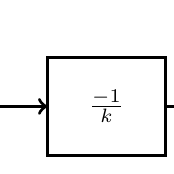
\begin{tikzpicture}[inner sep=0pt,outer sep=0pt,very thick,
sysblock/.style={draw,rectangle,inner sep=2pt,minimum width=1.5cm,minimum height=1.25cm,very thick}]
\useasboundingbox (-1,1) rectangle (0.5,-0.5); 
\begin{scope}[transform canvas={scale=1}]
\draw (0,0) node[sysblock] (S) {$\frac{-1}{k}$};
\draw[->] (-2,0) node[above=2pt] {$u$} -- (S.180);
\draw[->] (S.0) -- ++(1.5,0) node[above=2pt] {$y$};
\end{scope}
\end{tikzpicture}

	\end{center}
\end{frame}

We will go deeper into the mathematics of these block diagrams in future lectures; for now, the important things to remember are that we have input and output signals (variables) and systems represented by mathematical equations. 


\section{Examples}
\subsection{Example 1: Ideal elements for a car suspension}
Let's return to the car suspension system example. Each of the components can be represented by an ideal element, or combination of ideal elements that best represents the physical behavior. The exact configuration will  depend on the desired level of fidelity. However, a simple model is to take the car as a mass ($m_{c}$), the shock absorber as a damper ($b$), and the spring as a spring ($k$). The position of the wheel is determined by the road, and provides the boundary condition to the spring and damper $x_{r}$. The position of the car mass is indicated by $x_{c}$. 
\begin{frame}{Suspension system}
\begin{center}
\input{figures/autosuspension.tex}\hspace{.25in}\input{figures/autosuspensionmodel2.tex}
\end{center}
\end{frame}

\subsection{Example 2: Equations of motion for car suspension system}
In order to write down the equations of motion for a mechanical system, we can break the system apart to a {\em free body diagram} where each of the forces and positions relevant for each element can be explicitly exhibited. 
\begin{frame}{Free Body Diagram for Suspension System}
\begin{center}
\input{figures/autosuspensionmodel2fbd.tex}
\end{center}
\end{frame}
Note that we have added the effect of gravity as a downward force on the car mass, with magnitude $m_{c}g$, where $g$ is gravitational acceleration. In this free body diagram, we have been careful to draw the forces on the spring and damper components in the same way that they were defined in the component law. This will help us make sure that we get the signs on all of our terms correctly. Note, however, that the arrow only defines the direction of {\em positive} force. It does not necessarily mean that the force will always be in that direction - only that when the force is compressive, it will be considered positive.

Because the components are connected, many of the variables in the free body diagram are related. Usually, you can apply the connection laws directly when you draw the free body diagram. The result of applying the connection laws will be the following: 
\begin{frame}
\begin{center}
\begin{tikzpicture}

\draw[inner sep=0pt,outer sep=0pt,very thick] (2,0) node[rotate=90] (K1) {\begin{tikzpicture}
\draw (.75,0) node[inner sep=0,outer sep=0] (K1) {\begin{tikzpicture}
\draw (.75,0) node[inner sep=0,outer sep=0] (K1) {\input{\mainfolder/DrawingElements/MechanicalElements/spring.tex}};
\draw (K1)  node[above=6pt] {$k$};
\draw[very thick] (K1.180) -- ++(-.2,0);
\draw[very thick] (K1.0) -- ++(0.2,0);
\draw[<-,thick] (K1.0) ++(.2,0) -- ++(.5,0) node[right] {$f$};
\draw[<-,thick] (K1.180) ++(-.2,0) -- ++(-.5,0) node[left] {$f$};
\draw[|->,thick] (K1.180) ++(-.2,.4) node[above=2pt] {$x_{1}$} -- ++(.5,0);  
\draw[|->,thick] (K1.0) ++(.2,.4) node[above=2pt] {$x_{2}$} -- ++(.5,0);  
\draw<2-> (K1) ++(0,-.6) node {$f=k(x_{1}-x_{2})$};
\end{tikzpicture}
};
\draw (K1)  node[above=6pt] {$k$};
\draw[very thick] (K1.180) -- ++(-.2,0);
\draw[very thick] (K1.0) -- ++(0.2,0);
\draw[<-,thick] (K1.0) ++(.2,0) -- ++(.5,0) node[right] {$f$};
\draw[<-,thick] (K1.180) ++(-.2,0) -- ++(-.5,0) node[left] {$f$};
\draw[|->,thick] (K1.180) ++(-.2,.4) node[above=2pt] {$x_{1}$} -- ++(.5,0);  
\draw[|->,thick] (K1.0) ++(.2,.4) node[above=2pt] {$x_{2}$} -- ++(.5,0);  
\draw<2-> (K1) ++(0,-.6) node {$f=k(x_{1}-x_{2})$};
\end{tikzpicture}
};
\draw (K1) node[right=14pt] {$k$};
\draw[inner sep=0pt,outer sep=0pt,very thick] (-2,0) node[rotate=90] (D1) {\begin{tikzpicture}
\draw[very thick] (-.2,0) -- (0,0);
\draw (.75,0) node {\begin{tikzpicture}
\draw[very thick] (-.2,0) -- (0,0);
\draw (.75,0) node {\input{\mainfolder/DrawingElements/MechanicalElements/damper.tex}};
\draw (.75,0) node[above=9pt] {$b$};
\draw[very thick] (1.5,0) -- ++(.2,0);
    \draw[<-,thick] (1.5,0) ++(.2,0) -- ++(.5,0) node[right] {$f$};
    \draw[<-,thick] (-.2,0) -- ++(-.5,0) node[left] {$f$};
    \draw[|->,thick] (-.2,.4) node[above=2pt] {$x_{1}$} -- ++(.5,0);  
    \draw[|->,thick] (1.7,.4) node[above=2pt] {$x_{2}$} -- ++(.5,0);  
    \draw (.6,-.6) node {$x=x_{1}-x_{2}$};
  %  \draw (.6,-1.2) node {$f=b\dot{x}$};
\end{tikzpicture}};
\draw (.75,0) node[above=9pt] {$b$};
\draw[very thick] (1.5,0) -- ++(.2,0);
    \draw[<-,thick] (1.5,0) ++(.2,0) -- ++(.5,0) node[right] {$f$};
    \draw[<-,thick] (-.2,0) -- ++(-.5,0) node[left] {$f$};
    \draw[|->,thick] (-.2,.4) node[above=2pt] {$x_{1}$} -- ++(.5,0);  
    \draw[|->,thick] (1.7,.4) node[above=2pt] {$x_{2}$} -- ++(.5,0);  
    \draw (.6,-.6) node {$x=x_{1}-x_{2}$};
  %  \draw (.6,-1.2) node {$f=b\dot{x}$};
\end{tikzpicture}};
\draw (D1) node[left=14pt] {$b$};
\draw (0,3) node[draw,rectangle,minimum width=1.5cm,minimum height=1.5cm,very thick] (M1) {$m_{c}$};

\draw[|->] (K1.180) ++(-.35,-.25) node[left] {$x_{r}$} -- ++(0,.5);
\draw[|->] (K1.0) ++(-.35,.25) node[left] {$x_{c}$} -- ++(0,.5);
\draw[|->] (D1.180) ++(.35,-.25) node[right] {$x_{r}$} -- ++(0,.5);
\draw[|->] (D1.0) ++(.35,.25) node[right] {$x_{c}$} -- ++(0,.5);
\draw[|->] (M1) ++(1.25,0) node[right] {$x_{c}$} -- ++(0,.5);

\draw[very thick] (K1.180) -- ++(0,-.25) ;
\draw[very thick] (D1.180) -- ++(0,-.25) ;
\draw[very thick] (K1.0) -- ++(0,.25) ;
\draw[very thick] (D1.0) -- ++(0,.25) ;

\draw[<-] (M1.90) -- ++(0,.5) node[right] {$m_{c}g$};
\draw[<-] (K1.180) ++(0,-.25) -- ++(0,-.5) node[below] {$f_{k}$};
\draw[<-] (K1.0) ++(0,.25) -- ++(0,.5) node[above] {$f_{k}$};
\draw[<-] (D1.180) ++(0,-.25) -- ++(0,-.5) node[below] {$f_{b}$};
\draw[<-] (D1.0) ++(0,.25) -- ++(0,.5) node[above] {$f_{b}$};

\draw[<-] (M1.-90) ++(.25,0) -- ++(0,-.5) node[below] {$f_{b}$};
\draw[<-] (M1.-90)  ++(-.25,0) -- ++(0,-.5) node[below] {$f_{k}$};
\end{tikzpicture}

\end{center}
\end{frame}

\begin{frame}
\mode<presentation>{\begin{center}\resizebox{1in}{!}{\begin{tikzpicture}

\draw[inner sep=0pt,outer sep=0pt,very thick] (2,0) node[rotate=90] (K1) {\begin{tikzpicture}
\draw (.75,0) node[inner sep=0,outer sep=0] (K1) {\begin{tikzpicture}
\draw (.75,0) node[inner sep=0,outer sep=0] (K1) {\input{\mainfolder/DrawingElements/MechanicalElements/spring.tex}};
\draw (K1)  node[above=6pt] {$k$};
\draw[very thick] (K1.180) -- ++(-.2,0);
\draw[very thick] (K1.0) -- ++(0.2,0);
\draw[<-,thick] (K1.0) ++(.2,0) -- ++(.5,0) node[right] {$f$};
\draw[<-,thick] (K1.180) ++(-.2,0) -- ++(-.5,0) node[left] {$f$};
\draw[|->,thick] (K1.180) ++(-.2,.4) node[above=2pt] {$x_{1}$} -- ++(.5,0);  
\draw[|->,thick] (K1.0) ++(.2,.4) node[above=2pt] {$x_{2}$} -- ++(.5,0);  
\draw<2-> (K1) ++(0,-.6) node {$f=k(x_{1}-x_{2})$};
\end{tikzpicture}
};
\draw (K1)  node[above=6pt] {$k$};
\draw[very thick] (K1.180) -- ++(-.2,0);
\draw[very thick] (K1.0) -- ++(0.2,0);
\draw[<-,thick] (K1.0) ++(.2,0) -- ++(.5,0) node[right] {$f$};
\draw[<-,thick] (K1.180) ++(-.2,0) -- ++(-.5,0) node[left] {$f$};
\draw[|->,thick] (K1.180) ++(-.2,.4) node[above=2pt] {$x_{1}$} -- ++(.5,0);  
\draw[|->,thick] (K1.0) ++(.2,.4) node[above=2pt] {$x_{2}$} -- ++(.5,0);  
\draw<2-> (K1) ++(0,-.6) node {$f=k(x_{1}-x_{2})$};
\end{tikzpicture}
};
\draw (K1) node[right=14pt] {$k$};
\draw[inner sep=0pt,outer sep=0pt,very thick] (-2,0) node[rotate=90] (D1) {\begin{tikzpicture}
\draw[very thick] (-.2,0) -- (0,0);
\draw (.75,0) node {\begin{tikzpicture}
\draw[very thick] (-.2,0) -- (0,0);
\draw (.75,0) node {\input{\mainfolder/DrawingElements/MechanicalElements/damper.tex}};
\draw (.75,0) node[above=9pt] {$b$};
\draw[very thick] (1.5,0) -- ++(.2,0);
    \draw[<-,thick] (1.5,0) ++(.2,0) -- ++(.5,0) node[right] {$f$};
    \draw[<-,thick] (-.2,0) -- ++(-.5,0) node[left] {$f$};
    \draw[|->,thick] (-.2,.4) node[above=2pt] {$x_{1}$} -- ++(.5,0);  
    \draw[|->,thick] (1.7,.4) node[above=2pt] {$x_{2}$} -- ++(.5,0);  
    \draw (.6,-.6) node {$x=x_{1}-x_{2}$};
  %  \draw (.6,-1.2) node {$f=b\dot{x}$};
\end{tikzpicture}};
\draw (.75,0) node[above=9pt] {$b$};
\draw[very thick] (1.5,0) -- ++(.2,0);
    \draw[<-,thick] (1.5,0) ++(.2,0) -- ++(.5,0) node[right] {$f$};
    \draw[<-,thick] (-.2,0) -- ++(-.5,0) node[left] {$f$};
    \draw[|->,thick] (-.2,.4) node[above=2pt] {$x_{1}$} -- ++(.5,0);  
    \draw[|->,thick] (1.7,.4) node[above=2pt] {$x_{2}$} -- ++(.5,0);  
    \draw (.6,-.6) node {$x=x_{1}-x_{2}$};
  %  \draw (.6,-1.2) node {$f=b\dot{x}$};
\end{tikzpicture}};
\draw (D1) node[left=14pt] {$b$};
\draw (0,3) node[draw,rectangle,minimum width=1.5cm,minimum height=1.5cm,very thick] (M1) {$m_{c}$};

\draw[|->] (K1.180) ++(-.35,-.25) node[left] {$x_{r}$} -- ++(0,.5);
\draw[|->] (K1.0) ++(-.35,.25) node[left] {$x_{c}$} -- ++(0,.5);
\draw[|->] (D1.180) ++(.35,-.25) node[right] {$x_{r}$} -- ++(0,.5);
\draw[|->] (D1.0) ++(.35,.25) node[right] {$x_{c}$} -- ++(0,.5);
\draw[|->] (M1) ++(1.25,0) node[right] {$x_{c}$} -- ++(0,.5);

\draw[very thick] (K1.180) -- ++(0,-.25) ;
\draw[very thick] (D1.180) -- ++(0,-.25) ;
\draw[very thick] (K1.0) -- ++(0,.25) ;
\draw[very thick] (D1.0) -- ++(0,.25) ;

\draw[<-] (M1.90) -- ++(0,.5) node[right] {$m_{c}g$};
\draw[<-] (K1.180) ++(0,-.25) -- ++(0,-.5) node[below] {$f_{k}$};
\draw[<-] (K1.0) ++(0,.25) -- ++(0,.5) node[above] {$f_{k}$};
\draw[<-] (D1.180) ++(0,-.25) -- ++(0,-.5) node[below] {$f_{b}$};
\draw[<-] (D1.0) ++(0,.25) -- ++(0,.5) node[above] {$f_{b}$};

\draw[<-] (M1.-90) ++(.25,0) -- ++(0,-.5) node[below] {$f_{b}$};
\draw[<-] (M1.-90)  ++(-.25,0) -- ++(0,-.5) node[below] {$f_{k}$};
\end{tikzpicture}
}\end{center}}
\mode<article>{Now we can write down the component equations. Lets look at the mass first. Since both $f_{k}$ and $f_{b}$ are positive in the same direction as $x_{c}$ is positive, we use a positive sign in Newton's law.}
\[
m_{c}\ddot{x}_{c} = f_{k} +f_{b} - m_{c}g
\]
\mode<article>{For the spring and damper, we use a positive sign for $x_{r}$, as it is positive in the same direction that $f_{b}$ and $f_{k}$ are positive. Since $x_{c}$ points in the opposite direction, it is negative}
\begin{align*}
f_{b} &= b(\dot{x}_{r} - \dot{x}_{c})\\
f_{k} &= k(x_{r} - x_{c})
\end{align*}
\end{frame}

\begin{frame}
\mode<article>{We can now find the relationship between any two variables of interest. For example, we can find the differential equation relating $x_{r}$ and $x_{c}$ by plugging in $f_{b}$ and $f_{k}$}
\[
m_{c}\ddot{x}_{c} = k(x_{r} - x_{c})+ b(\dot{x}_{r} - \dot{x}_{c}) - m_{c}g
\]
or
\[
m_{c}\ddot{x}_{c} +b\dot{x}_{c} +kx_{c}= kx_{r} +b\dot{x}_{r} - m_{c}g
\]
\end{frame}
\section{Application Example}

An active prosthetic device can help people with amputations live better. The word ``active'' here means that the prosthetic is actively controlled via a feedback control system. One example of an active prosthetic is given in the article\\

\noindent Samuel Au, Jeff Weber, Hugh Herr, ``Powered Ankle-Foot Prosthesis Improves Walking Metabolic Economy,'' \textit{IEEE Trans. on Robotics}, Vol. 25, No. 1, Feb. 2009.\\

\noindent which begins (emphasis added):

\begin{quotation}
	"Abstract - At moderate to fast walking speeds, the human ankle provides net positive work at high-mechanical-power output to propel the body upward and forward during the stance period. On the contrary, conventional ankle-foot prostheses exhibit a passive elastic response during stance, and consequently, cannot provide net work. 
	\textbf{Clinical studies indicate that transtibial amputees using conventional prostheses have higher gait metabolic rates than normal.}
	Researchers believe that the main cause for these higher rates is due to the inability of conventional prostheses to provide sufficient positive power at terminal stance in the trailing leg to limit heel strike losses of the adjacent leading leg. In this investigation, we evaluate the 
	\textbf{hypothesis that a powered ankle-foot prosthesis, capable of providing human-like ankle work and power during stance, can decrease the metabolic cost of transport (COT) compared to a conventional passive-elastic prosthesis.}" (p. 1)
\end{quotation}

The abstract points to a problem experienced by people with transtibial (lower leg) amputations, namely that they may require more energy to walk because some prosthetics are inefficient. Can engineering improve these prosthetics?\\


The following three figures appear in (Au, 2009) and illustrate the prosthetic from side view and with an ideal element representation consisting of masses, springs, a motor, and a transmission:


\begin{center}
	\includegraphics[width=3.5in]{figures/ProstheticFoot.png}
\end{center}

\begin{center}
	\includegraphics[width=2in]{figures/ProstheticModel.png}
\end{center}

The new, active prosthetic can be modeled with ideal elements (such as mass, spring, and damper) and a feedback control loop can be constructed to optimize it for the user.

\begin{center}
	\includegraphics[width=4.5in]{figures/FeedbackControlLoop.png}
\end{center}


\section{Lecture Highlights}
The primary takeaways from this article include
\begin{enumerate}
\setlength{\itemsep}{5pt}
\setlength{\parskip}{0pt}
\setlength{\parsep}{0pt}
\item A physical system that we are interested in controlling can be modeled as a ``plant'' within a feedback control loop. This feedback loop includes \textit{systems} (represented by blocks) and \textit{signals} (represented by arrows). The signals are variables, such as the room temperature in the thermostat feedback control system diagram, and the systems are mathematical relationships between variables (e.g., differential equations).
\item Physical systems can be represented by idealized components such as masses, springs, and dampers that have component laws. Components are connected mathematically using connection rules.
\end{enumerate}

\section{Quiz Yourself}

\subsection{Questions}
\begin{enumerate}
\setlength{\itemsep}{5pt}
\setlength{\parskip}{0pt}
\setlength{\parsep}{0pt}
\item Find the differential equation(s) that describe the following systems:
\begin{enumerate}
\item \rule{0pt}{12pt}\\
\begin{center}
\input{quizfigures/massspringdamper1.tex}
\end{center}
\item \rule{0pt}{12pt}\\ 
\begin{center}
\input{quizfigures/massspringdamper2.tex}
\end{center}
\item \rule{0pt}{12pt}\\ 
\begin{center}
\input{quizfigures/massspringdamper3.tex}
\end{center}
\end{enumerate}
\item You are training for a water skiing competition. In order to better your performance, you want to model the velocity of the water skier. Note that the rope stretches when tension is applied, but also exhibits some characteristics of a damper.
\begin{enumerate}
\item What are the input and output of the system?
\item Draw a model using idealized elements
\item Find the differential equations describing this system.
\end{enumerate}
\begin{center}
\includegraphics[width=4in]{quizfigures/waterskiier}
\end{center}
\end{enumerate}

\subsection{Solutions}

\begin{enumerate}
\setlength{\itemsep}{5pt}
\setlength{\parskip}{0pt}
\setlength{\parsep}{0pt}
\item \rule{0pt}{12pt}\\
\begin{enumerate}
\item \rule{0pt}{12pt}\\
\begin{center}
\includegraphics[width=5in]{quizfigures/1asoln}
\end{center}\newpage
\item \rule{0pt}{12pt}\\ 
\begin{center}
\includegraphics[width=5in]{quizfigures/1bsoln}
\end{center}
\item \rule{0pt}{12pt}\\ 
\begin{center}
\includegraphics[width=5in]{quizfigures/1csoln}
\end{center}
\end{enumerate}\newpage
\item \rule{0pt}{12pt}\\ 
\begin{center}
\includegraphics[width=6in]{quizfigures/2soln}
\end{center}
\end{enumerate}

\section{Resources}

\subsection{Books}
Since there are many applications of control to mechanical systems, techniques for modeling these systems can be found in almost all introductory controls textbooks. Some textbooks introduce Laplace Transforms first, but the following textbook also incorporates direct use of differential equations, as discussed in this lecture.

\begin{itemize}
\item Gene F. Franklin, J. David Powell and Abbas Emami-Naeini,  {\em Feedback Control of Dynamic Systems}, Pearson
\begin{itemize}
\item 6th and 7th edition: section 2.1
\end{itemize}
\end{itemize}


\subsection{Web resources}
There are also some web resources that cover mechanical systems. If you find something useful, or if you find a link that no longer works, please inform your instructor!

\begin{itemize}
\item \url{https://www.youtube.com/watch?v=MN3RJWcJKnk}. This is very complete (1 hour) video from Rick Hill at University of Detroit, Mercy. This covers both translational and rotational mechanical systems, including gear trains. (We will not discuss gear trains in these notes, but they are very common in rotational mechanical systems)

\end{itemize}



\end{document}


